
\documentclass[11pt]{article}

\usepackage{graphicx, amsmath, amsfonts, amssymb, amsxtra, bm}
\usepackage[usenames,dvipsnames]{xcolor}
\usepackage[protrusion=true, expansion=true]{microtype}
\usepackage[authoryear]{natbib}
\usepackage[font={small}, bf]{caption}
\usepackage[T1]{fontenc}
\usepackage[utf8]{inputenc}
\usepackage[a4paper, margin=1in]{geometry}
\usepackage{txfonts}
\usepackage{xr}

\newcommand{\SI}{SI}
\newcommand{\ud}{\text{d}}
\newcommand{\mat}[1]{\bm{#1}}
\newcommand{\cov}{\text{cov}}
\newcommand{\rem}[1]{\textcolor{red}{\textrm{#1}}}
\newcommand{\citeapos}[1]{\citeauthor{#1}'s (\citeyear{#1})}
\let\originalleft\left
\let\originalright\right
\renewcommand{\left}{\mathopen{}\mathclose\bgroup\originalleft}
\renewcommand{\right}{\aftergroup\egroup\originalright}
\newcommand{\FdL}[1]{\textcolor{Cerulean}{\textrm{#1}}}
\renewcommand{\thefigure}{R\arabic{figure}}
\renewcommand{\thetable}{R\arabic{table}}
\renewcommand{\theequation}{R\arabic{equation}}
\newcommand{\us}{\rm \setlength{\leftskip}{0.3cm} \setlength{\rightskip}{0.3cm}}
\newcommand{\them}{\it \setlength{\leftskip}{0cm} \setlength{\rightskip}{0cm}}


\setlength{\parskip}{0.8em}
\setlength{\parindent}{0em}
\bibpunct{(}{)}{,}{a}{}{,}
\clubpenalty = 10000
\widowpenalty = 10000
\graphicspath{{../../../SI/}}
\externaldocument[SI:]{../appendix}
\externaldocument[main:]{../manuscript}


\begin{document}

\begin{flushright}
  Dr.~John Drake\\
  Senior Editor\\
  Ecology Letters
\end{flushright}


\begin{flushleft}
\textbf{Manuscript number: } \texttt{ELE-00187-2020} \\
``A Bayesian network approach to trophic metacommunities shows habitat loss accelerates top species extinctions''\\
Johanna H\"aussler, Gy\"orgy Barab\'as \& Anna Eklöf
\end{flushleft}


Dear Dr.~Drake,

Thank you for your consideration of our submission, and the chance to revise and resubmit our manuscript to \textit{Ecology Letters}. We additionally thank Dr.~Gravel and the anonymous reviewer for their thoughtful engagement with our work and valuable suggestions. Please see our detailed point-by-point responses to each of their comments below.

Apart from a few minor changes, the main text has been left mostly intact compared with the previous version. However, we have made substantial new additions to the Supporting Information (\SI) based on the requests from the Reviewers. In particular, we have:
\begin{itemize}
\item Relaxed the assumption that the conditional probability of consumer extinction is strictly a function of the fraction of its resource species that are absent. We now also consider weighted Bayesian networks, where the importance of each prey species to the consumer's diet may be different (\SI, Section~\ref{SI:sec:weighted}).
\item Reproduced published results on the maximum possile number of trophic levels a landscape can sustain, given some of its properties like the number of patches and the average distance between them. The published study \citep{Ryser2019} uses a fully-fledged dynamical metacommunity approach based on the Allometric Trophic Network model. Our simpler, Bayesian network-based results not only match those of the more complicated model qualitatively, but yield analytical insight into why such patterns arise in the first place.
\item Further explored the role of space and spatial arrangement of habitat patches, by repeating our patch removal analyses both on random landscapes and ones with a regular layout of patches in a two-dimensional grid (and also landscapes that were in between these two extremes). It turns out that metacommunities tend to be more fragile when the landscape is highly regular, with random landscapes leading to higher metapopulation capacities.
\item Implemented the removal of links between pairs of patches, instead of the patches themselves. As in the case of patch removal, we compared the scenarios of removing the most- and least valuable landscape connections first, and a scenario of random link removal. While results are similar to what we see with patch removal, there is an important difference: the adverse effects of random link removal on metacommunity persistence are in between the best- and worst-case ones (whereas in the case of patch removal, the random scenario was practically indistinguishable from the worst-case one).
\end{itemize}


We point out all additional changes in our detailed responses to the Reviewers below. Thank you once again for your time.

\bigskip

Best regards,

Johanna H\"aussler, Gy\"orgy Barab\'as \& Anna Eklöf

\newpage


\section*{Response to reviewer comments}

\subsection*{Reviewer 1}

\them

This paper presents a new modelling approach for predicting patterns of occupancy in bottom-up driven trophic metacommunities. This novel approach uses Bayesian networks to predict which species should persist in each patch on a landscape, given an assumed dispersal model and functional form for how local extinction risks should depend on the fraction of prey resources available to each predator. The authors demonstrate how to use this approach to estimate the effect of habitat restrictions in four scenarios assuming different patterns of baseline mortality and dispersal, and under three different scenarios of habitat remove. The authors also demonstrate what patterns of habitat loss this model would predict for a terrestrial food web, parameterized using predator-prey relationships from a Serengeti food web data set.

The author's approach to developing the Bayesian network model is rigorously constructed, and carefully explained. I found the thorough discussion of the method in box 1 and in S1 to be very helpful, and I think this approach has the potential to be very useful for modelling extinction scenarios across landscapes. However, I do have one substantial concern with the paper, as well as some more minor comments.

\us

We thank the Reviewer for the exceptionally careful reading of our manuscript, the detailed comments, the encouragement, and the constructive criticism and helpful suggestions for improvement.

\them

My primary concern is that the Bayesian network model makes several strong assumptions about ecological interactions, and there is no evidence given in the paper to determine whether those assumptions are justified based on evidence from real food webs, or to assess how robust the predictions of extinction patterns are to violations of those assumptions. The primary results of the paper, that extinction rates will generally increase with trophic level and with removing highly connected habitats, are in line with the broader literature on spatial patterns of extinction. This model may be very useful for making quantitative predictions for large food webs and for identifying critical habitats to protect, but for that to be the case, it is important that it is able to accurately predict extinction patterns. Any model that is useful for understanding specific cases should be validated either by showing it makes accurate specific conditions, or that the assumptions the model is based on are consistent with empirical facts \citep{IvesAgrawal2005}.

\us

This is a very important point, and in response, we have obtained several new results to emphasize 1) their robustness; and 2) that predicted extintion patterns resemble those obtained via other methods. These were done to move beyond the broad but simple agreement of our results with existing literature mentioned by the Reviewer, to see if the model can be used more quantitatively. To this end, we have relaxed the assumption that each prey item contributes a fixed fraction to predators' diets, and show that results are robust to abandoning this assumption. We have also reproduced the predictions for the number of trophic levels as a function of landscape size and number of patches from a different study \citep{Ryser2019} which took both bottom-up and top-down effect into account. The patterns produced by the two methods are qualitatively identical. See below for details.

\them

One of the core assumptions of the author's model is that extinction risk depends functionally on the fraction of a species' total resources that are available within a given patch. I am not aware of any ecological research on how extinction risk might vary with the fraction of prey available to a predator, and this particular assumption does have an odd consequence; it means that if there are two otherwise equivalent species, but one of the species is able to prey on an additional resource that happens to be absent from a patch, that more generalist species will be more likely to go extinct than the first one. An alternative assumption would be that extinction risk would depend on the absolute number of resources available within a patch, but I suspect the model would show very different patterns of extinction. I would recommend that the authors include either strong empirical evidence for the justification the current functional form, or a supplementary analysis to show that the predicted outcomes are robust to the assumption.

\us

The scenario envisioned by the Reviewer above might not be as strange as it looks. It means that we are tacitly assuming some sort of tradeoff between predator efficiency and generality. In the example above: if the specialist consumer preys on two resources available in the patch, and the generalist on three (but the third is locally absent), then, since the generalist is less efficient overall, it is at a disadvantage compared to the specialist.

While such explanations are plausible, there is of course no telling how commonly they would apply without a detailed study of the natural history of the organisms involved. Fortunately, the extinction risk depending only on the fraction of prey lost is not so much a core assumption, but rather a methodological choice. It can easily be relaxed. We have now done so, re-doing the patch removal analysis with a weighted trophic network, where the contribution of each prey item to the persistence of its consumers depends on species identity. The relative importance of resource $j$ to consumer $i$, $\theta_{ji}$, is the proportion of biomass flowing from $j$ to $i$ per unit time relative to the other resources. We obtained the entries $\theta_{ji}$ of the flow matrix as the corresponding entry of the Jacobian matrix of the allometric trophic network model \citep{Schneider2016, Ryser2019}, evaluated at equilibrium. Repeating the patch removal analysis using these weighted feeding networks resulted in the same outcome as the original, purely fraction-dependent ones. See the new Section~\ref{SI:sec:weighted} in the Supporting Information (\SI) for the detailed results and methodology.

Additionally, to emphasize that the assumption of conditional extinction probabilities being a function of the fraction of prey lost is a methodological choice and not a core assumption, we have revised the Box in the main text and Section~\ref{SI:sec:BN} in the \SI.

\them

A second core assumption of this model is that extinction risks only depend on bottom-up effects. While the authors are careful to note this limitation (page 14 line 14) and recommend that if ``in a given system, top-down effects are deemed important, other methods should be used instead'', there is no guidance on when top-down effects are expected to be important, and the model used here has not been demonstrated to be able to accurately predict extinction patterns in the presence of potential top-down effects. I would recommend a comparison of spatial extinction patterns predicted by the Bayesian network approach to those predicted by a dynamical metacommunity model, as used in \citet{Ryser2019}, to verify if this approach produces qualitatively similar extinction patterns compared to a dynamic model.

\us

This is an excellent suggestion. Figure~S2 in \citet{Ryser2019} shows the maximum number of trophic levels of a food web that were able to persist, given the average patch distance and the number of patches. We have re-created this figure using our Bayesian network approach (Figure~\ref{fig:Ryser_repr}). The results are qualitatively unchanged, with a strong dependence of the maximum attainable trophic level on the spatial scale, and a weaker one on the number of patches.

Moreover, this case study can also be used to highlight another advantage of our method: due to its analytical tractability, it is possible to get a deeper understanding of its results. Approximating trophic networks as trophic chains, assuming a common baseline extinction probability $\pi_i = \pi$, and using the patch-averaging method described in our \SI, Section~\ref{SI:sec:chain}, we have $T \approx \lambda_M \log(\pi^{-1})$, where $T$ is the maximum number of trophic levels and $\lambda_M$ is the dominant eigenvalue of the dispersal matrix (Eq.~\ref{main:eq:Tapprox} in our main text). Obtaining these eigenvalues for each of the landscapes used in Figure~\ref{fig:Ryser_repr}, we can depict this approximation (Figure~\ref{fig:Ryser_semianal}). This figure looks very much like Figure~S2 in \citet{Ryser2019}, and it is based on the fully tractable approximation $T \approx \lambda_M \log(\pi^{-1})$. This lends further credence to the idea that the pattern observed here and in \citet{Ryser2019} is not contingent on model details, but is a robust logical consequence of combining trophic interactions and metacommunity structure.

We present and discuss these results in Section~\ref{SI:sec:ryser} of the \SI.

\begin{figure}[!p]
  \centering
  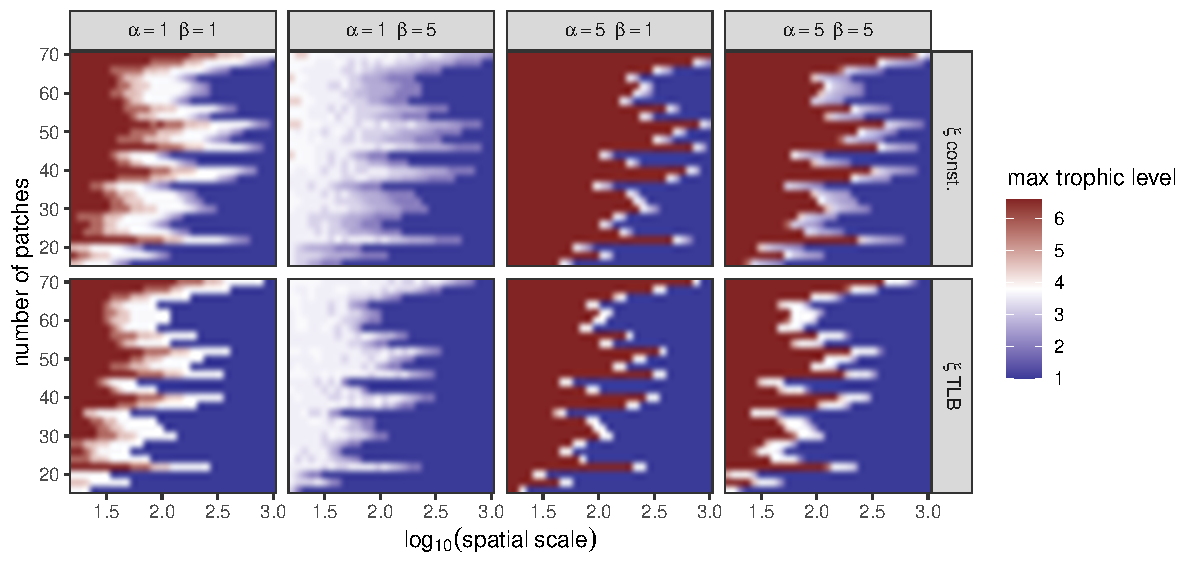
\includegraphics[width=\textwidth]{Ryser_reproduced.pdf}
  \caption{The maximum number of trophic levels (colors) persisting on a landscape with different numbers of patches (ordinate) and average distance between them (abscissa). The web we used, which had 50 basal and 350 consumer species, was the same as the one in the main text. In the top row, each species has an identical dispersal parameter $\xi$ (equal to the spatial scale indicated along the abscissa), while in the bottom row, they were trophic level-based (increasing linearly with trophic level such that their average was equal to the spatial scale parameter). Columns show various parameterizations of the consumer response to prey loss (linear, convex, concave, and sigmoid). The results are qualitatively identical to Figure~S2 in \citet{Ryser2019}: there is a strong dependence of the maximum attainable trophic level on the spatial scale, and a weaker one on the number of patches.}
  \label{fig:Ryser_repr}
\end{figure}

\begin{figure}[!p]
  \centering
  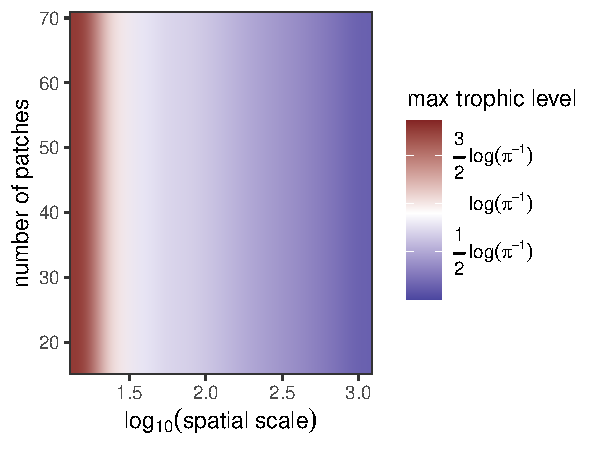
\includegraphics[width=0.65\textwidth]{Ryser_semianalytic.pdf}
  \caption{Analytical approximation of the expected maximum number of trophic levels (colors), given species' dispersal ability (abscissa) and the number of patches in the landscape (ordinate). The heat map is based on the approximation $T \approx \lambda_M \log(\pi^{-1})$ (Eq.~\ref{main:eq:Tapprox} in the main text), with the leading eigenvalues of the landscapes explicitly calculated based on their associated dispersal matrices.}
  \label{fig:Ryser_semianal}
\end{figure}

\them

Other notes:

Page 4, line 55: It would have been useful to me to have the broad model assumptions stated in text prior to the formal model description, especially the assumptions that extinction rates only depend on the number of available resources (not presence of competitors or prey), and that extinction rates varied with fraction of available resources.

\us

We have now added an introductory paragraph outlining the core model assumptions, before diving into the details (lines ...).

\them

Page 5 line 5: The notation is a bit confusing here. $M^{kl}_i$ is stated to be a species-specific landscape matrix, but from the equation it is clear that it is the k-by-l'th entry of a specific matrix.

\us

Now we say they are modeled using a species-dependent landscape matrix, whose $(k,l)$th entry $M_i^{kl}$ gives the dispersal rate of species $i$ from patch $l$ to patch $k$ (lines ...).

\them

Page 5, line 9-12: this text is a bit unclear, as it is confusing an extinction rate with a probability. A probability of extinction only makes sense in a specific time frame. It is also unclear what is meant by ``the first term of a Poisson distribution''. I would recommend rephrasing this along the lines of ``within-patch extinction is modelled as a Poisson process with a rate $E_i^k$, so the probability of extinction occurring within one time period is $\delta_i^k = 1- \exp(-E_i^k)$, from which [\ldots]''.

\us

We have rewritten the sentence in the suggested way (lines ...).

\them

Page 6, line 43:56: why are these in a different order than in the figure? For instance, why does \#1 on this list correspond to figure 2C, whereas \#2 corresponds to figure 2A?

\us

We have changed the ordering to match the list. We now always follow this order: linear ($\alpha = \beta = 1$), convex ($\alpha = 5$, $\beta = 1$), concave ($\alpha = 1$, $\beta = 5$), and sigmoid ($\alpha = \beta = 5$).

\them

Page 8, line 52: ``In the best-case scenario, unless consumer response to prey absence is described by a strongly concave function'': this should refer to a specific panel figure 2.

\us

We have added the subfigure reference (subpanel C; lines ...).

\them

Page 9, line 18: dispersal rates may not always increase with trophic level, and may actually decrease in some ecosystems \citep{Pedersenetal2016}. For instance, \citet{Beisneretal2006} show evidence that higher trophic level species (zooplankton, fish) in lakes disperse more rarely than smaller organisms based on community dissimilarity patterns, and \citet{Villarinoetal2018} show the same phenomenon with plankton based on body sizes.

\us

This is a fair point---we have added a paragraph discussing that this assumption need not hold in all systems (lines ...).

\them

Page 11, line 18: Why was this specific species chosen?

\us

It is the only basal species that is also the sole member of a spatial group. So it was a natural choice. But there is no need to do this; in fact, we have done the analysis with another basal species' patch rankings (see Figure~\ref{fig:ser} below; Figure~\ref{SI:S_fig:patchloss_Serengeti_SGB_alt} in the revised \SI). As seen, the results are qualitatively unchanged.

\begin{figure}[!ht]
\centering
\hspace{-5em}
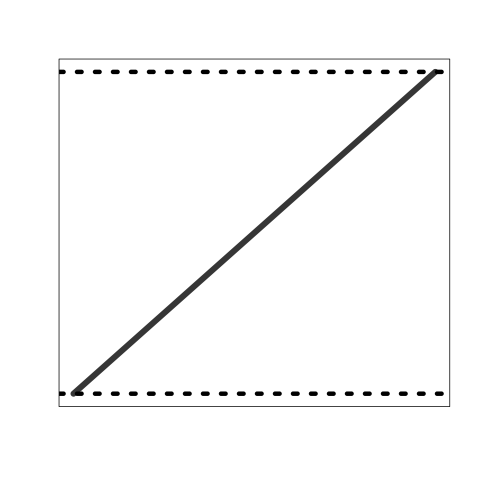
\includegraphics[width=0.2\textwidth]{fform_1_1.png}
\hspace{0.5em}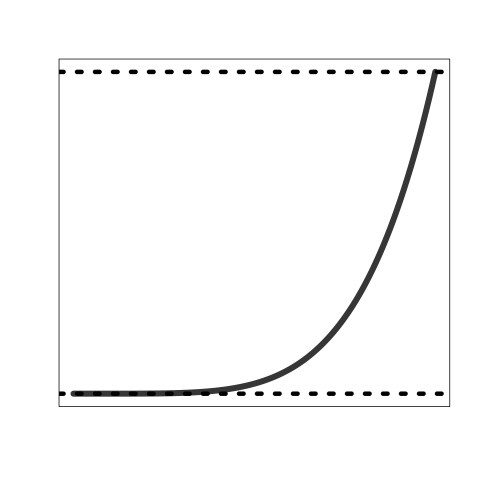
\includegraphics[width=0.2\textwidth]{fform_5_1.png}
\hspace{0.5em}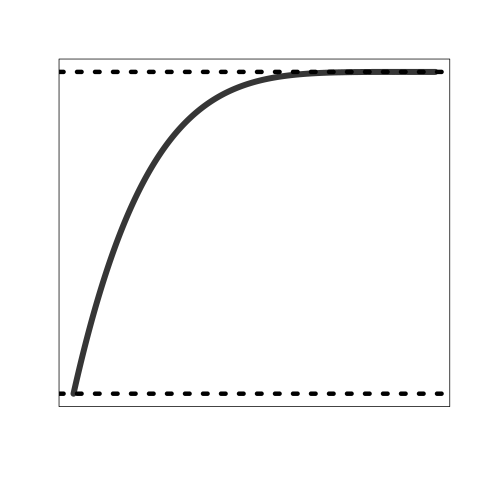
\includegraphics[width=0.2\textwidth]{fform_1_5.png} \hspace{0.5em}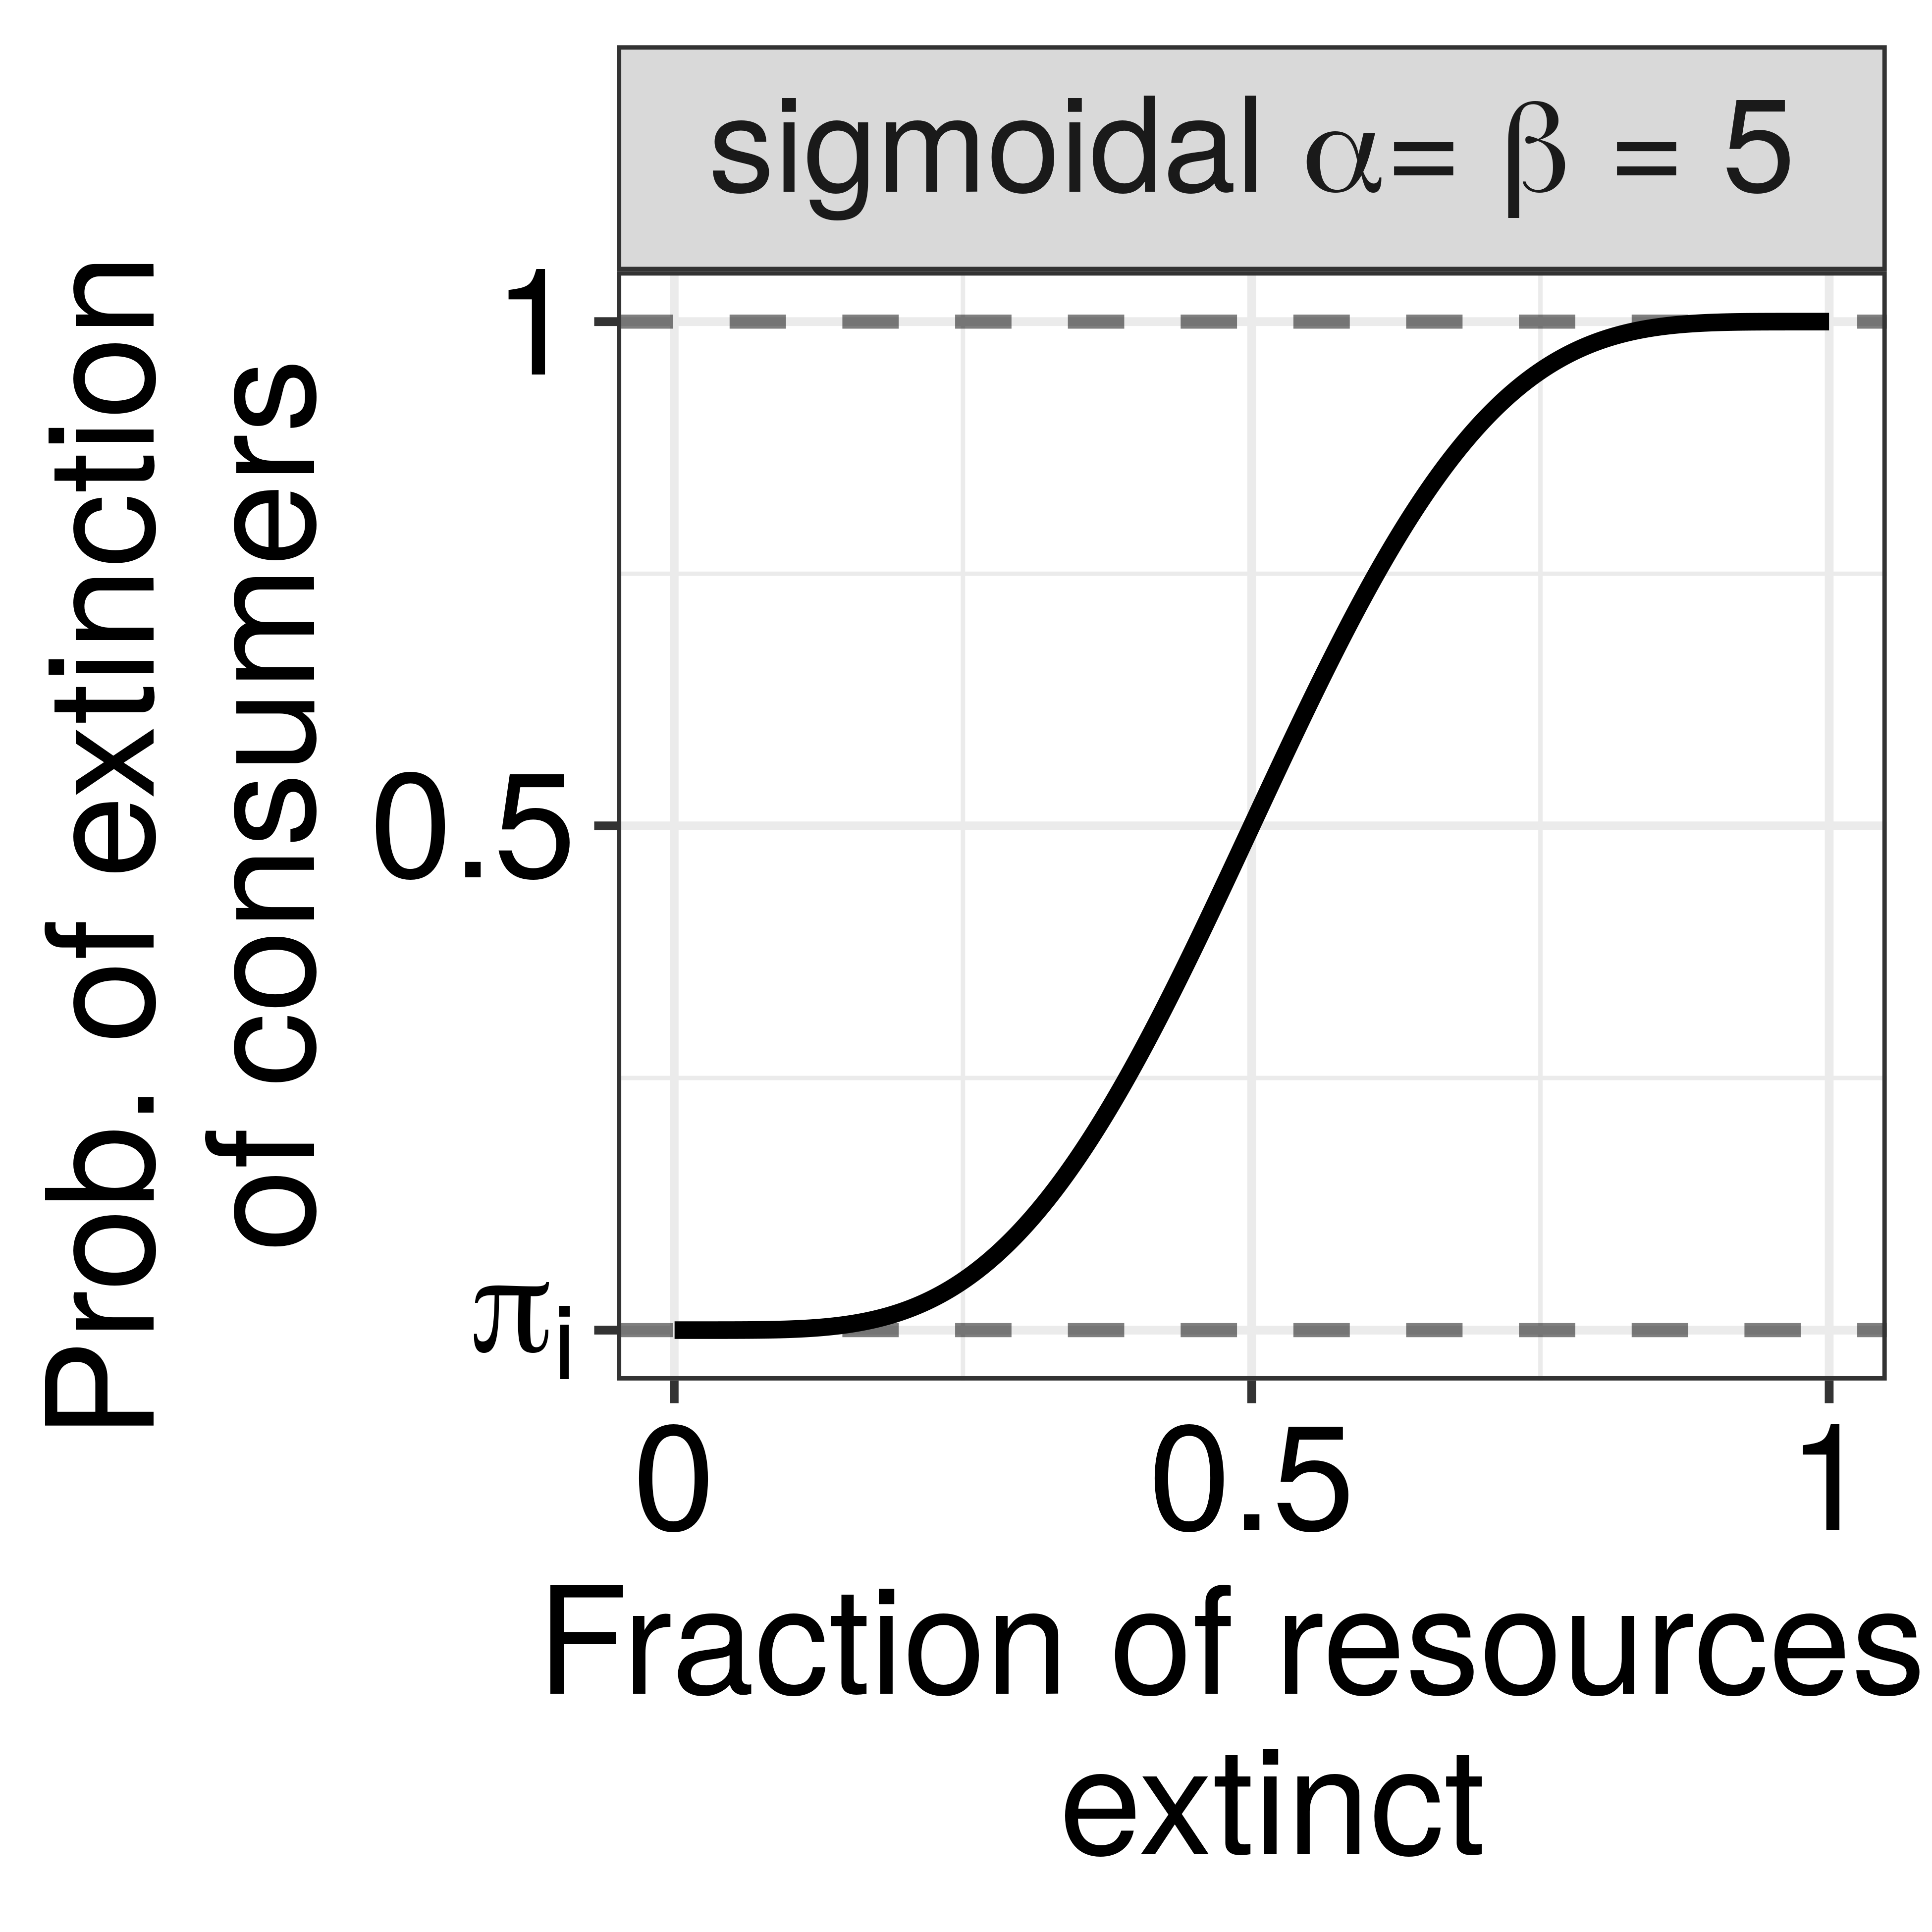
\includegraphics[width=0.2\textwidth]{fform_5_5.png}

\vspace{1.5em} 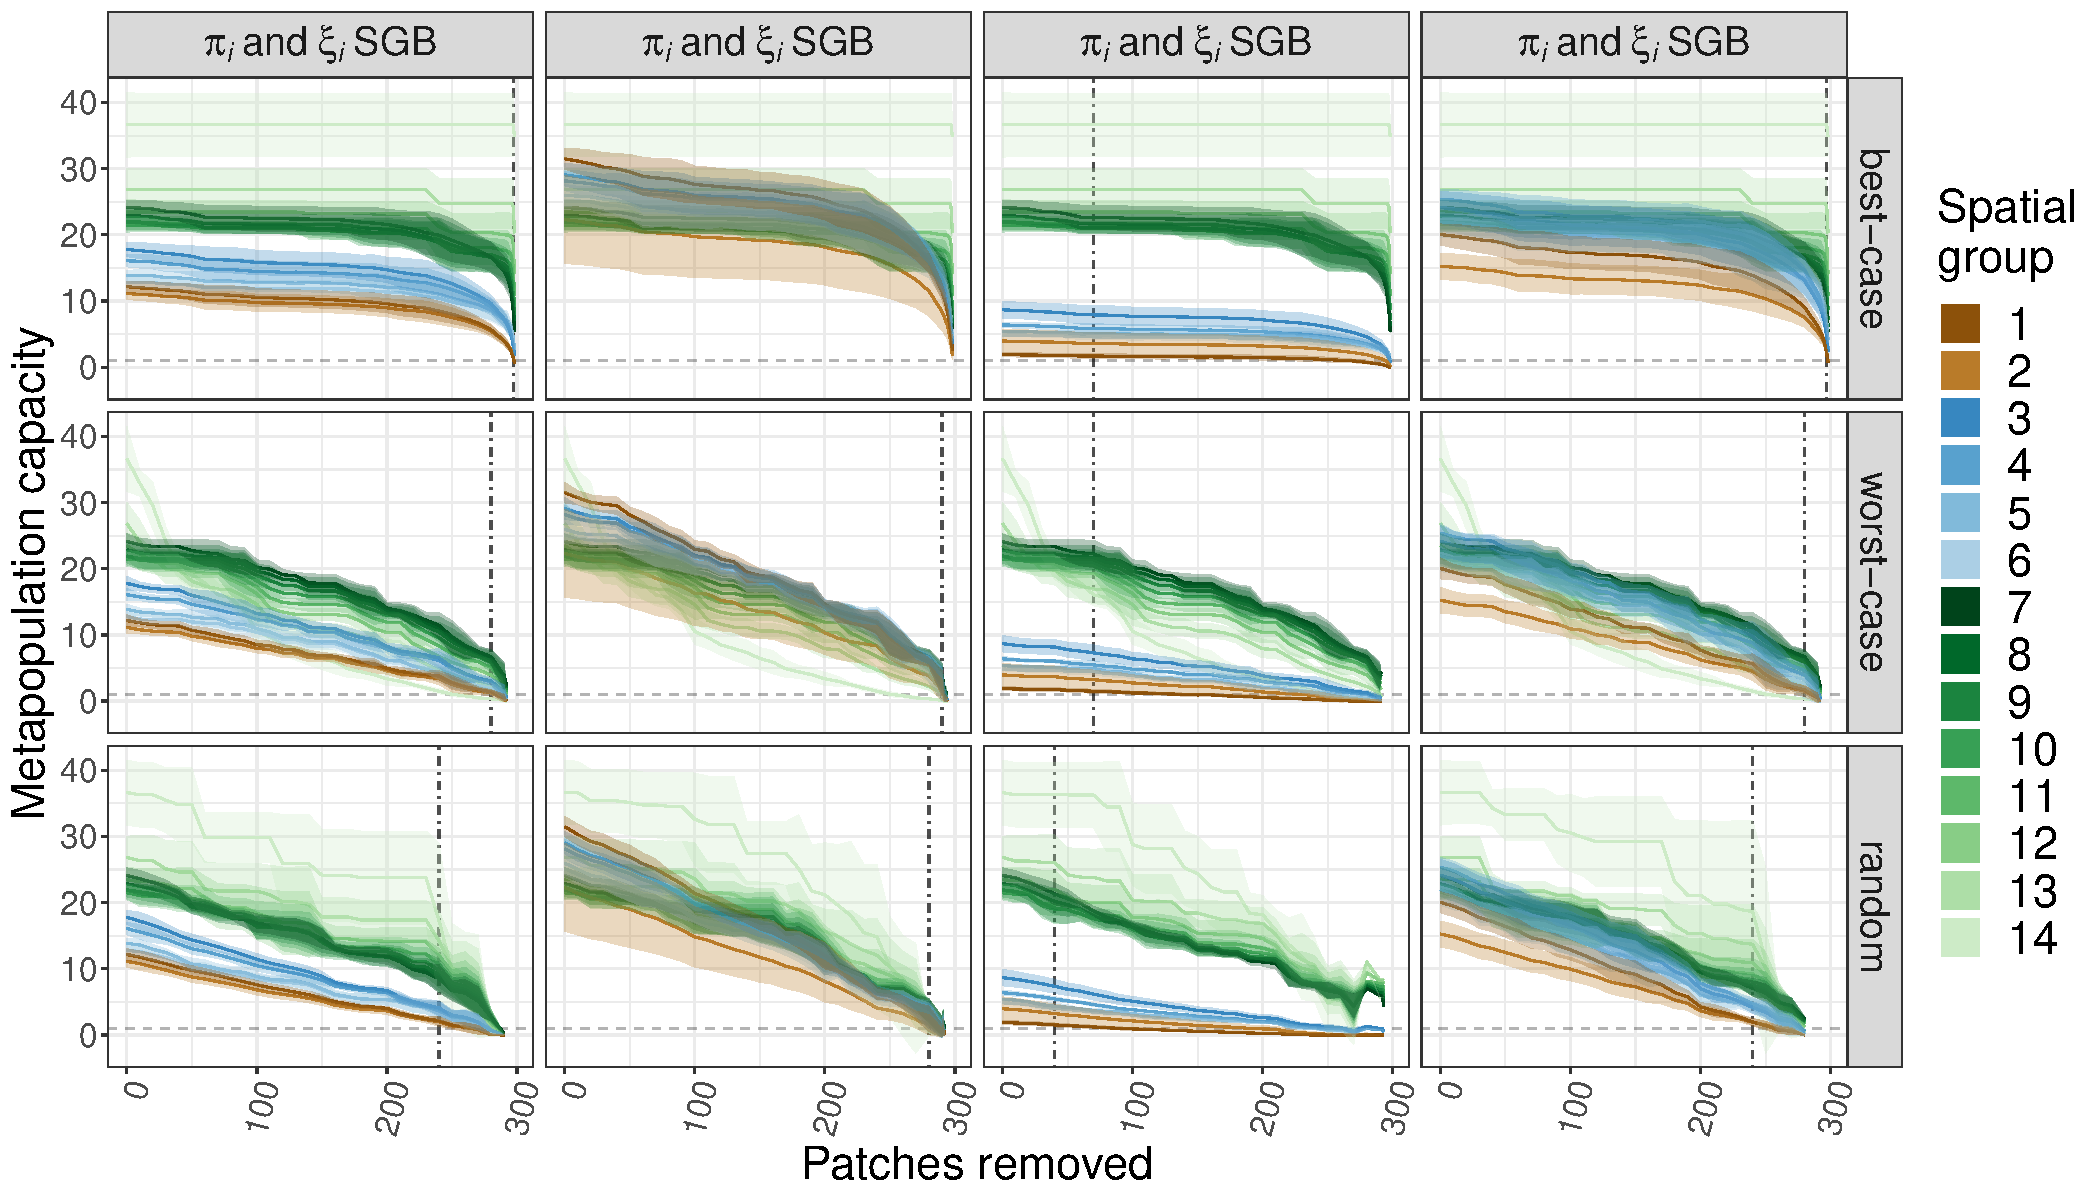
\includegraphics[width=\textwidth]{lambda_Serengeti_food_web_with_32_consumer_and_129_basal_species_basal_SGB_BOSAUG.pdf}
\caption{As Figure~4 in the main text, except the species whose metapopulation capacity serves as the basis of patch removal is different. In the main text, this species was the Gum arabic tree (\textit{Acacia senegal}), the sole representative of spatial group 12. Here, we have instead chosen a species from spatial group 14, \textit{Boscia augustifolia}. Results are qualitatively unchanged by this alteration.}
\label{fig:ser}
\end{figure}

\them

Page 14, line 25: It is also important to note another limitation of this approach; the calculation of extinction rates depends very heavily on the assumption of the separation of time scales between extinction and colonization, as the Bayesian network method of calculating extinction probability assumes that there is no chance of an extinction cascade within a patch being stopped by a colonist of a prey species arriving midway through; i.e. mass effects are also assumed not to play a role in extinction dynamics. This approach also explicitly assumes that everything is in (quasi)equilibrium when calculating local extinction rates, so likely will not work to calculate e.g. extinction debts or out-of-equilibrium patch occupancy dynamics.

\us

This is indeed the case; we now discuss this in lines ...

\them

Figure 2: I would recommend labelling the axes of the insets. Currently, the functional forms show how extinction risk changes with fraction of prey items missing, but a causal reader could easily infer that they represent probability of survival with fraction of prey present, as the natural ordering for the x-axis would be to range from 0\% of prey available to 100\% of prey available. I would also recommend only plotting integer trophic levels (rather than the fractional trophic levels), as the extra lines make the figure more visually difficult to understand, without giving extra information on the dynamics.

\us

We have revised the figure insets and changed the plot to show integer trophic levels (we did the same in all corresponding figures in the \SI\ as well). Please note that, as per the recommendation of Reviewer 2 (Dr.~Gravel), we have changed the order of Figures~2 and 3, so the relevant figure is now Figure~2 in the main text.

\them

S1, page 1: B(f) refers to the extinction probability as a function of the number of resources, but the appendix also discusses a specific species, B. This means that equation S2 and S3 are needlessly confusing to understand; I would suggest using different notation for the function B(f). 

\us

Good point---we have changed the notation from $B(f)$ to $w(f)$ (suggesting that it is a \emph{w}eighting function) in both the main text and the \SI.

\them

S1, page 2: ``In this quasi-equilibrium state, there is some constant probability of going extinct'': this is unclear; does this mean there is some constant rate of extinction per unit time, or some constant probability of a given species being extinct at any given point in time? Is it the probability of going extinct before the arrival of the next colonist? Also, it would help to clarify that this means local (within patch) extinction, as the focus of the paper is on how metacommunity dynamics may affect that rate of global extinctions.

\us

We have revised Section~\ref{SI:sec:tmm} of the \SI\ to clarify both that the rate of going extinct is constant through time, and that this refers to local extinction.

\them

S1 page 2, equation S9: I think this relates to my previous question; I may be missing something here, but I don't understand why the probability of patch occupancy for a given prey species is multiplied by one minus their probability of persistence in the patch. Naively, it seems like the probability that a prey is not present in a patch is given simply by $(1-p_{\text{prey}}^k)$, given that has already been found iteratively based on the resources present below it in the food web. If $\delta_R^k$ is the probability of going extinct in a fixed period (where it's assumed that no colonization events take place) then the current notation makes sense (i.e. if a focal species only has one prey item, it will go extinct in a given time period if it's prey is not present at the start of a time period (dependent on $p_{\text{prey}}^k$) or if that prey item goes extinct during the period ($\delta_R^k$) but this needs to be clarified in text.

\us

The Reviewer is entirely correct: we assume constant rates, which then lead to constant probabilities \emph{per unit time}, which we have not mentioned explicitly. We have rewritten Section~\ref{SI:sec:tmm}, and also cast Eq.~\ref{SI:eq:bayesprob} in a different form to clarify this.

\them


\subsection*{Reviewer 2 (Dominique Gravel)}

This manuscript reports an investigation of the effect of habitat loss in a trophic metacommunity model. The model is a natural extension of previous ones used to investigate the effect of spatial dynamics on food web structure. Consumers are subject to colonization and extinction dynamics following a spatially explicit representation of Levins' model, with the additional feature that their extinction rate increases with the lost of prey. It builds on the Bayesian network representation of interactions to represent interaction mediated extinctions. The main analysis consists of removing patches and exploring the fraction of persisting species according to different scenarios. The main conclusions are that higher trophic levels are more sensitive to habitat loss and that some patches are more important than others to maintain metapopulation capacities.

I particularly appreciated certain aspects of the model : 

\begin{itemize}
\item It generalizes previous approaches using the spatially explicit formulation of Hanski and collaborators of the Levins model;
\item It nicely integrates a technique of network robustness analysis within a metacommunity framework, allowing a smoother representation of extinction probabilities and sequences;
\item It accounts for size/trophic level variation in colonization and extinction probabilities (in agreement with conclusions of Guzman et al.)
\end{itemize}
That said, there are also (known and acknowledged) limitations of the model :
\begin{itemize}
\item Only extinction depends on interactions, while previous models and a an empirical analysis (Cirtwill and Stouffer, 2015 GEB) have shown that both that it could also impact colonization;
\item The analysis (as most robustness analyses too) relies only on a bottom-up view of the world, neglecting potential effects of trophic cascades and indirect interactions on extinctions.
\end{itemize}

\us

We thank Dr.~Gravel for his very thorough reading or our work and the constructive suggestions for improvement. We respond to his points below.

\them

The manuscript itself is very well prepared, I do not have specific comments other than figure 3 should appear before figure 2.

\us

We have changed the order of the figures.

\them

My overall feeling is that this study could be a nice and welcome contribution to metacommunity ecology, but that several lines of investigation could be developed further to take advantage of the strengths of the modelling approach. As it is, most of the results could have been derived from previous trophic metacommunity models. A good example of this is Figure 3, which is basically the same result obtained by Holt in several of his contributions to island biogeography and \citet{Calcagnoetal2011} who generalized this theory later. I don't mean that Figure 3 is useless, but the analysis of metapopulation capacity could further build on the spatially explicit nature of the model. For instance, landscapes with aggregated patches could be compared and see how it influences lambda for different trophic levels with different dispersal distances. 

\us

These are all very good points. Apart from mentioning the work of \citet{Calcagnoetal2011} in relation to the maximum number of trophic levels being limited by metacommunity structure alone (lines ...), we have also added a new analysis, comparing a gradient of landscapes ranging from a perfectly grid-like patch arrangement to random ones.

We created this gradient by starting out with a $18\times 18$ perfect two-dimensional grid of patches, and then jiggling the position of each patch by adding a uniform random value to both their x- and y-coordinates. The range in which the random addition happens ranges from $0$ (perfect grid) to $\pm 0.5$. Since the landscape is assumed to be in the unit square, coordinate values over $1$ and below $0$ were wrapped around to appear on the other side of the landscape. E.g., an x-coordinate of $1.2$ was treated as being $0.2$. We then performed the same patch removal analysis as before on each of these landscapes, for the case of $\alpha = \beta = 1$ (linear consumer response to prey loss). We recorded, for each scenario and parameterization, the number of patches that must be removed for the species of a given trophic level to disappear. Results are in Figure~\ref{fig:gridlike} (Section~\ref{SI:sec:gridlike} in the updated \SI). What we see is that very regular grids of patches lead to more vulnerable species, with fewer patches needing removal to drive them extinct. (The lines are noisy, because we have only generated a single landscape with a given level of grid perturbation. Averaging results over multiple landscapes would smooth them out.) The reason random landscapes are better is that they have, by chance, clusters of close-by patches, boosting species' metapopulation capacities. Note though that there are diminishing returns: beyond a point, making  the landscapes even more aggregated no longer enhances persistence, as seen from the figure.

\begin{figure}[!ht]
  \centering
  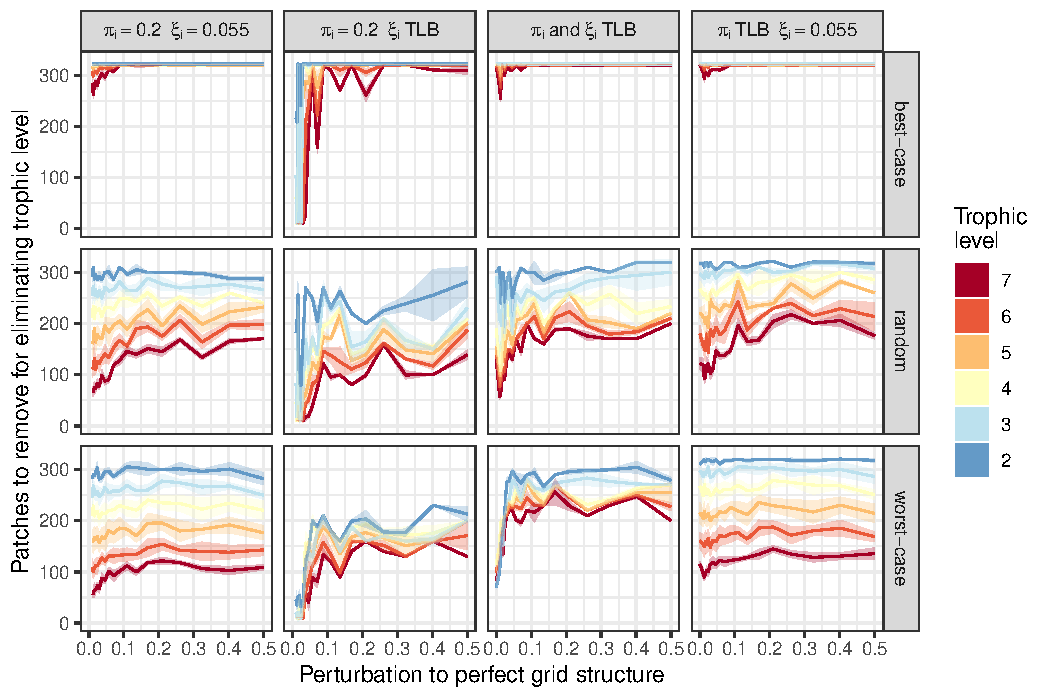
\includegraphics[width=0.95\textwidth]{gridlike.pdf}
  \caption{The number of patches (ordinate) which, when removed, cause the extinction of species at various trophic levels (colors, with the lines showing the mean across the species of each trophic level, and the bands around it the one-sigma standard deviations). The abscissa shows how far the patches of the landscape are from being perfectly arranged in a grid ($0$: perfect grid; $0.5$: random landscape). We see that more grid-like landscapes lead to lower persistence thresholds, but that landscapes above a perturbation level of about $0.2$ behave as if they were completely random.}
  \label{fig:gridlike}
\end{figure}


\them

What follows are suggestions, it is up to the authors to decide what to do with them :

- I think that the most original contribution of the study is the inclusion of explicit space following Hanski's work on metapopulation capacity. But unfortunately the analysis does not build on it, the same results could have been derived using a island-mainland approach (again, nothing in Figure 3 is taking advantage of explicit space). There are several ways to build on this, among them :

* Contribution of individual patches to metapopulation carrying capacity could be explored;
  
\us

We are grateful for these suggestions, because they indeed drive more attention to the advantages of having a spatially explicit framework. In relation to the specific comment above, we have in fact done just this when we removed patches in the best and worst possible sequence. To determine these, we evaluated the contribution of each patch to the metapopulation capacity of a basal species (and also a top predator, in Section~\ref{SI:sec:tsfs}). So in that sense we were already building on the spatially explicit nature of our model: the ranking of patches for their importance of metacommunity maintenance would not have been possible with any spatially implicit approach. Thus, Figures~\ref{main:fig:loss_example}, \ref{main:fig:patchloss}, and \ref{main:fig:Serengeti} in the main text do take spatial configuration into account.

\them

* Only dispersal links in the spatial network could be removed, allowing an analysis of fragmentation in addition to habitat loss

\us

This was a very good suggestion, one that produced interesting results. We have redone our analyses by removing, instead of randomly chosen patches, randomly chosen links between pairs of patches. Once a link is removed between two patches, no species can travel between them, regardless of their dispersal ability. We compared the outcome of this random link removal experiment with the random patch removal. Just as before, we have done best-case, worst-case, and random removal scenarios (\SI, Section~\ref{SI:sec:linkrem}). The results are qualitatively the same as with patch removal, but with one important exception: the random removal scenario now lies about mid-way between the best- and worst-case ones. This is in contrast with patch removal, where random removal was as bad as the worst-case scenario. We now mention this new result in the main text as well (lines ...).

\them

- The analysis could also build further on how Bayesian networks are used to study represent extinction sequences:

* It would be interesting to define a ``metacommunity robustness'' index, similar to the robustness analysis of topological networks (e.g. the amount of habitat loss a metacommunity could stand before 50\% of the species are going extinct). This index could be calculated for the whole food web and perhaps per trophic level, since higher trophic levels will have lower robustness

\us

The problem is that such a metric would give different robustness values depending on landscape layout, order of patch removal, and so on. (Comparing the point at which top predators go extinct in Figure~\ref{main:fig:patchloss} shows just how sensitive it is to the sequence in which we dispose of patches, for example.) For this reason, there is probably no universally useful, single metacommunity robustness index, but rather a suite of indices depending on spatial patch aggregation, whether patch removal is random, etc., which together may help give an intuitive feel for for fragile a given metacommunity is under various types of disturbances. While this direction is definitely interesting, we feel that its magnitude is beyond the scope of our work, so we decided not to pursue it further here.

\them

* Further, it would be interesting to compare the extinction sequence that is observe if one conduct a traditional node deletion numerical experiment vs a patch removal experiment. Are species extinctions following the same sequence ? At the same rate ? Such an analysis (which is easy to run) would provide a more process-based interpretation of extinction sequences, a common critique of such analyses.

\us

While we have not done a systematic analysis of this, it is certain that the extinction sequence from node deletion would be quite different from patch removal. With patch removal, all species are affected to an extent, but the adverse effects are cumulatively felt by species at higher trophic levels. As seen from our results, there is a reasonably well-groomed sequence to the disappearance of species at different trophic levels (Figure~\ref{main:fig:patchloss} in the main text), with higher levels going extinct first. With species removal, we could see many more basal species (or generally, those at lower levels) go extinct first, as long as they are not critical to the maintenance of the food web as a whole. As we said, we have not explored this in any greater detail, but would be happy to come back to it if Dr.~Gravel felt this would be a needed addition.

\them

- I also have two technical remarks about the representation of how interactions impact extinction:

* A smoother and conceptually similar way to account for the cumulative effects of prey availability on extinction probability was introduced before by \citet{Cazellesetal2015}. The formulation in this model, inspired by Lotka-Volterra equations, is not as elegant and computationally efficient as a Bayesian network, but it has the advantage of integrating variation in the contribution of each species to function B(f).

\us

We are grateful for the pointer to \citet{Cazellesetal2015}, which we now mention in the Discussion (lines ...). As we have written to Reviewer 1, the assumption that each prey species contributes equally to predator persistence can be relaxed in our framework, and we have now done so (\SI, Section~\ref{SI:sec:weighted}). To be consistent with this possibility, we have also revised the Box in the main text and Section~\ref{SI:sec:tmm} to treat the assumption of equal prey contribution as just a particular methodological choice, and not as a core assumption of our approach.

\them

* Further, I disagree with the interpretation that it is impossible to have a top-down effect in Bayesian representation of interactions (P14). Equation B1 could easily be modified such that it is the number of predators that is influencing the baseline extinction rate, instead of the number (or fraction) of prey. Again, \citet{Cazellesetal2015} implemented both in their formulation.

\us

This is of course true: the Bayesian network can be turned around an applies ``upside down'' to implement top-down effects. One problem though is that it is difficult to justify a biologically relevant form of conditional prey persistence as a function of predator extinction. For prey and their resources, things are clear: no consumer can persist without a food source. However, this is not so clear-cut the other way round. Should prey extinction likelihood increase or decrease with the number of consumer species? If it increases, then are we ignoring the fact that apparent competition can be reduced via predator-partitioning? And if it decreases, then are we saying that having more predator species ravaging a prey makes it less likely to be hunted to extinction? Without committing to any of these options, we merely highlight that implementing top-down effects raises important methodological problems which must first be resolved.

In response to this comment, we did change our text to no longer say that top-down effects are impossible to implement. Instead, we point out that it would not be a straightforward exercise to do so (lines ...).

\them


\section*{Comments from the Editor}

The authors have greatly interested two reviewers who nonetheless have some rather substantial criticisms. If these can be satisfactorily addressed (and the novelty and generality of the proposed method clearly established), the work could be published in Ecology Letters.

\us

Thank you for your consideration of the manuscript, and the chance to revise and resubmit our work. Please see our detailed responses to the Reviewers above, and the summary of major changes we have made on the top page. We have included several new results both to showcase the applicability of our method to a variety of problems (especially to be able to capitalize on its spatially explicit nature, in line with the suggestions of Dr.~Gravel), and to demonstrate its robustness against relaxing model assumptions.

\them \rm


\newpage
\bibliographystyle{../elsarticle-harv}
\bibliography{../biblio}


\end{document}

